\chapter{Théorie des ensembles et des applications}
\label{chap:ensembles}
\minitoc
\minilof
\minilot

La théorie des ensembles comprend l'étude des ensembles, l'étude de leurs parties et l'étude de leurs interactions grâce aux applications. On s'intéresse particulièrement aux injections, aux surjections et aux bijections. La troisième section présente les relations binaires comme la relation d'ordre ou la relation d'équivalence. La quatrième et dernière section se focalise sur les familles d'éléments comme par exemple des suites. 

Ce chapitre est primordial dans le programme de MPSI, il décrit le langage nécessaire pour travailler de manière sérieuse en mathématiques.
%
\section{Vocabulaire relatif aux ensembles}
\label{chap3-sec:vocabensemble}
Nous prenons comme notion primitive les notions d'ensemble, d'élément et d'appartenance. On ne cherchera pas à les définir, \og\(x \in E\)\fg{} sera lu \og \emph{l'élément \(x\) appartient à l'ensemble \(E\)} \fg{}.
%
\subsection{Égalité de deux ensembles}
\label{chap3-subsec:egalitededeuxensembles}
\begin{defdef}
  On dira que deux ensembles \(E\) et \(F\) sont égaux si ils ont les mêmes éléments. On notera \(E=F\),
  \begin{equation}
    E=F \iff \forall x \quad \left(x \in E \iff x \in F \right).
  \end{equation}
\end{defdef}
%
\subsection{Inclusion}
\label{chap3-subsec:inclusion}
\begin{defdef}
  Soient \(E\) et \(F\) deux ensembles. On dira que \(E\) est inclus dans \(F\) ou que \(E\) est un sous-ensemble de \(F\) si et seulement si tous les éléments de \(E\) sont des éléments de F. On notera \(E \subset F\)
\end{defdef}
\begin{prop} 
  \begin{equation}
    E=F \iff E \subset F \textrm{~et~} F \subset E.
  \end{equation}
\end{prop}
Pour dire que \(E\) est strictement inclus dans \(F\) c'est à dire \(E \subset F \textrm{~et~} F \not\subset E\), on notera \(E \subsetneq F\)
\begin{equation}
  E \subsetneq F \iff \left[\forall x \quad \left(x \in E \iff x \in F \right) \right] \textrm{~et~} \left[\exists x \in F \quad x \not\in E \right].
\end{equation}
%
\subsection{Ensemble des parties d'un ensemble}
\label{chap3-subsec:ensembledesparties}
\begin{axiome}[Axiome de l'ensemble des parties]
  Soit un ensemble \(E\). Il existe un ensemble dont les éléments sont les parties de \(E\). On l'appelle ensemble des partie de \(E\) et il est noté \(\Part(E)\) et
\begin{equation}
  A \in \Part(E) \iff A \subset E.
\end{equation}
\end{axiome}
Il n'y a que deux autres façons de définir un ensemble~:
\begin{itemize}
\item en extension, c'est-à-dire qu'on énumère les éléments de l'ensemble, par exemple \(S=\{1;2;3\}\) ;
\item en compréhension, c'est-à-dire qu'on définit l'ensemble \(E\) comme sous-ensemble d'un ensemble plus grand. Le sous ensemble des éléments de \(F\) qui vérifie une certaine propriété, par exemple l'ensemble des entiers pairs de \(\Z\), \(E_1=\enstq{n\in\Z}{\exists k \in \Z \quad n=2k}\).
\end{itemize}
%
\subsection{Opérations sur les parties d'un ensemble}
\label{chap3-subsec:operationparties}
Soient \(E\) un ensemble, \(A\) et \(B\) des parties de \(E\). On définit les opérations sur les ensembles \(A\) et \(B\) suivantes
décrites dans les paragraphes suivants.
%
\subsubsection{Complémentaire de \(A\) dans \(E\)} 
\label{chap3-subsubsec:complementaire}
C'est l'ensemble de \(E\) qui ne sont pas des éléments de \(A\), noté \(\complement_E A\) ou \(\bar{A}\)~\footnote{ne pas confondre avec l'adhérence, cf programme de MP} ou \(E \setminus A\).
\begin{equation} 
  \forall x \in E \quad x \in \complement_E A \iff x \not\in A.
\end{equation}
Le diagramme de Venn correspondant est donné par la figure~\ref{chap3-fig:comp}.
%
\begin{figure}
\centering
\begin{tikzpicture}
\draw \En; 
\fill[pink] \An; 
%\fill[green, opacity=0.2] \Bn;
\draw (-4,-1) node[above right]{\(E\)}; 
\draw (-2,0) node{\(A\)}; 
\draw (0,-0.5) node{\(\bar{A}\)}; 
%\draw (2,0) node{\(B\)};
\end{tikzpicture}
\caption{Représentation du complémentaire}
\label{chap3-fig:comp}
\end{figure}
%
\begin{prop}
  Soient \(A\) et \(B\) deux parties de \(E\)
  \begin{gather}
  \complement_E (\complement_E A)=A; \label{eq:comp1}\\
  A \subset B \iff \complement_E B \subset \complement_E A. \label{eq:comp2}
  \end{gather}
\end{prop}
\begin{proof}
    Prouvons \eqref{eq:comp1}. Soit \(a \in E\), \(a \in \complement_E (\complement_E A)\) équivaut à \(a \not\in \complement_E A\) ; ce qui équivaut à \(a \in A\). Prouvons la première implication de \eqref{eq:comp2}. Soit \(x \in \complement_E B\) alors \(x \not\in B\), alors par hypothèse, \(A \subset B\), \(x\) ne peut pas être dans \(A\), \(x \not\in A\), donc \(x\) est dans le complémentaire de \(A\)~: \(x \in \complement_E A\).

    Prouvons la deuxième implication de \eqref{eq:comp2}. Soit \(x \in A\), alors \(x \not\in \complement_E A\), alors par hypothèse, \(\complement_E B \subset \complement_E A\), \(x\) ne peut pas être dans \(\complement_E B\), \(x \not\in \complement_E B\), donc par définition du complémentaire, \(x \in B\).
\end{proof}
%
\subsubsection{Intersection des parties \(A\) et \(B\)}
\label{chap3-subsubsec:intersection}
C'est l'ensemble des éléments qui sont à la fois dans \(A\) et dans \(B\), on le note \(A \cap B\),
\begin{equation}
  \forall x \in E \quad x \in A \cap B \iff x \in A \text{~et~} x \in B.
\end{equation}
Le diagramme de Venn correspondant est donné par la figure~\ref{chap3-fig:inter}.

\begin{figure}
\centering
\begin{tikzpicture}
\draw \En; 
\fill[red, opacity=0.2] \An; 
\fill[green, opacity=0.2] \Bn;
\fill[blue, opacity=0.5] \AnB;
\draw (-4,-1) node[above right]{\(E\)}; 
\draw (-2,0) node{\(A\)}; 
\draw (2,0) node{\(B\)};
\draw (0,2) node{\(A \cap B\)};
\end{tikzpicture}
\caption{Représentation de l'intersection}
\label{chap3-fig:inter}
\end{figure}

\subsubsection{Réunion des parties \(A\) et \(B\)}
\label{chap3-subsubsec:reunion}
C'est l'ensemble des éléments qui appartiennent au moins à l'une des parties \(A\) et \(B\), on le note \(A \cup B\).
\begin{equation}
  \forall x \in E \quad x \in A \cup B \iff x \in A \text{~ou~} x \in B
\end{equation}
Le diagramme de Venn correspondant est donné par la figure~\ref{chap3-fig:reunion}.

\begin{figure}
\centering
\begin{tikzpicture}
\draw \En; 
\fill[red, opacity=0.2] \An; 
\fill[green, opacity=0.2] \Bn;
\fill[blue, opacity=0.5] \AuB;
\draw (-4,-1) node[above right]{\(E\)}; 
\draw (-2,0) node{\(A\)}; 
\draw (2,0) node{\(B\)};
\draw (0,2) node{\(A \cup B\)};
\end{tikzpicture}
\caption{Représentation de la réunion}
\label{chap3-fig:reunion}
\end{figure}

\subsubsection{Différence de A et B}
\label{chap3-subsubsec:difference}
C'est l'ensemble des éléments de \(E\) qui appartiennent à \(A\) mais pas à \(B\), noté \(A \setminus B\).
\begin{gather}
  \forall x \in E \quad x \in A \setminus B \iff x \in A \text{~et~} x \not\in B; \\
  A \setminus B=A \cap \complement_E B.
\end{gather}
Le diagramme de Venn correspondant est donné par la figure~\ref{chap3-fig:diff}.

\begin{figure}
\centering
\begin{tikzpicture}
\draw \En; 
\fill[red, opacity=0.2] \An; 
\fill[green, opacity=0.2] \Bn;
\fill[blue, opacity=0.5] \AmB;
\draw (-4,-1) node[above right]{\(E\)}; 
%\draw (-2,0) node{\(A\)}; 
\draw (2,0) node{\(B\)};
\draw (-2,2) node{\(A \setminus B\)};
\end{tikzpicture}
\caption{Représentation de la différence \(A \setminus B\)}
\label{chap3-fig:diff}
\end{figure}

\subsubsection{Différence symétrique de \(A\) et \(B\)}
\label{chap3-subsubsec:differencesymetrique}
C'est l'ensemble des éléments de \(E\) qui appartiennent à exactement une des parties \(A\) et \(B\), on le note $A \Delta
B$~:
\begin{equation}
  \forall x \in E \quad x \in A \Delta B \iff x \in A \cup B \text{~et~} x \not\in A \cap B.
\end{equation}
Le diagramme de Venn correspondant est donné par la figure~\ref{chap3-fig:diffsym}.

\begin{figure}
\centering
\begin{tikzpicture}
\draw \En; 
\fill[red, opacity=0.2] \An; 
\fill[green, opacity=0.2] \Bn;
\fill[blue, opacity=0.5] \AmB;
\fill[blue, opacity=0.5] \BmA;
\draw (-4,-1) node[above right]{\(E\)}; 
%\draw (-2,0) node{\(A\)}; 
%\draw (2,0) node{\(B\)};
\draw (-1,2) node{\(A \Delta B\)};
\end{tikzpicture}
\caption{Représentation de la différence symétrique \(A \Delta B\)}
\label{chap3-fig:diffsym}
\end{figure}

\begin{prop}
  Soient \(A\) et \(B\) des parties de \(E\), on a 
  \begin{gather}
    A \Delta B = (A\setminus B) \cup (B \setminus A) = (A \cap \bar{B}) \cup (B \cap \bar{A}); \\
    A \Delta B =(A \cup B) \setminus (B \cap A) = (A \cup B) \cap \bar{A \cap B} =(A \cup B) \cap (\bar{A} \cup \bar{B})
  \end{gather}
\end{prop}

\subsubsection{Propriétés}
\label{chap3-subsubsec:prop}
\begin{axiome}
  Soient \(A, B\) et \(C\) trois parties de \(E\), on a les axiomes suivants respectivement~:
  \begin{itemize}
    \item La commutativité
        \begin{gather}
            A \cap B= B \cap A, \\  
            A \cup B=B \cup A;
        \end{gather}
    \item l'associativité
        \begin{gather}
            A \cap (B \cap C)=(A \cap B) \cap C, \\ 
            A \cup (B \cup C)=(A \cup B) \cup C;
        \end{gather}
    \item la distributivité
        \begin{gather}
            A \cap (B \cup C)=(A \cap B) \cup (B \cap C), \\ 
            A \cup (B \cap C)=(A \cup B) \cap (A \cup C);
        \end{gather}
    \item la stabilité
        \begin{gather}
            A \subset B \implies (A \cap C) \subset (B \cap C), \\ 
            A \subset B \implies (A \cup C) \subset (B \cup C);
        \end{gather}
    \item les lois de De Morgan
        \begin{gather}
            \complement_E (A \cup B)=\complement_E A \cap \complement_E B, \\ 
            \complement_E (A \cap B)=\complement_E A \cup \complement_E B;
        \end{gather}
    \item les lois de Boole
        \begin{gather}
            A \cap (A \cup B)=A, \\ 
            A \cup (A \cap B)=A.
        \end{gather}
    \end{itemize}
\end{axiome}
%
\subsection{Ensemble vide}
\label{chap3-subsec:ensemblevide}
Si \(E\) est un ensemble, \(\complement_E E\) est la seule partie de \(E\) sans élément. On l'appelle la partie vide de \(E\). Si \(F\) est un autre ensemble, on a \(\complement_E E = \complement_F F\). On parlera de l'ensemble vide de \(E\) au lieu de dire la partie vide de \(E\), on le note \(\emptyset\). Quelque soit l'ensemble \(E\), \(\complement_E E =\emptyset\).

Faire attention à ne pas confondre \(\emptyset = \{\}\) qui ne contient rien avec \(\{\emptyset\}\) qui contient l'ensemble
vide.

\subsection{Produit cartésien de deux ensembles}
\label{chap3-subsec:prodcart}
\begin{defdef}
  Pour deux éléments \(x\) et \(y\) de \(E\), on appelle couple \((x,y)\) la partie \(\{\{x\},\{x;y\}\}\). C'est un artifice pour se donner les éléments dans un certain ordre.
\end{defdef}
%
\begin{prop}
  Soient quatre éléments de \(E\), \(x\) ,\(y\), \(x'\) et \(y'\) alors 
  \begin{equation} 
    (x,y)=(x',y') \iff \begin{cases} x=x' \\ y=y' \end{cases}.
  \end{equation}
\end{prop}
\begin{proof}
Supposons que \(x=x'\) et \(y=y'\), alors 
\begin{equation}
  (x,y)=\{\{x\},\{x,y\}\}=\{\{x'\},\{x',y'\}\}=(x',y').
\end{equation}
Si on suppose maintenant que \((x,y)=(x',y')\) alors 
\begin{equation}
  \{\{x\},\{x,y\}\}=\{\{x'\},\{x',y'\}\}.
\end{equation}
Par l'absurde, si \(x \neq x'\) on a \(\{x\}=\{x',y'\}\) et \(\{x,y\} = \{x'\}\) donc \(x'=y'=x\) et \(y=x'=x\) donc on aboutit à la contradiction \(x=x'\). Nécessairement \(x'=x\) et donc \(y=y'\).
\end{proof}
%
\begin{defdef}
  Soient \(E\) et \(F\) deux ensembles, on appelle produit cartésien de \(E\) et \(F\), qu'on note \(E \times F\) l'ensemble $E
  \times F = \enstq{(x,y)}{x \in E \ y \in F}$.
\end{defdef}
Si \(E=F\) alors on note \(E \times E=E^2\). Si on dispose de \(n\) ensemble \(E_k\), on définit par récurrence le produit \(\prod_{k=1}^n E_k\) et les n-uplets \((x_k)\).

\section{Application}
\label{chap3-sec:applications}
\subsection{Notion d'application}
\label{chap3-subsec:notiondapplication}
\begin{defdef}
  On appelle application tout triplet \((E, F, \Gamma)\) où \(E\) et \(F\) sont des ensembles, \(\Gamma\) une partie de \(E \times F\) telle que 
  \begin{equation}
    \forall x \in E \ \exists! y \in F \quad (x,y) \in \Gamma.
  \end{equation}
\end{defdef}
Une représentation graphique de la notion d'application est donné sur la figure~\ref{chap3-fig:application}. Soit une
application \(f=(E,F,\Gamma)\), alors \(E\) est l'ensemble de départ, \(F\) celui d'arrivée et \(\Gamma\) est le graphe de \(f\).
Pour un élément \(x \in E\), soit \(y\) l'unique élément de \(F\) tel que \((x,y) \in \Gamma\) alors \(y\) est l'image de \(x\) par
l'application \(f\) et \(x\) est l'antécédent de \(y\) par \(f\). On écrit \(y=f(x)\). On note \(\fonction{f}{E}{F}{x}{f(x)}\) et on dit que \(f\) est une application de \(E\) dans \(F\). On note \(F^E\) l'ensemble des applications de \(E\) dans \(F\).
%
\begin{defdef}
  Soient \(f=(E,F,\Gamma)\) et \(g=(E',F',\Gamma')\) deux applications, on dit que \(f=g\) si \(E=E'\), \(F=F'\) et \(\Gamma=\Gamma'\).
\end{defdef}
Dans le cas où on sait déjà que \(E=E'\) et \(F=F'\), on a
\begin{equation}
  f=g \iff \forall x \in E \quad f(x)=g(x).
\end{equation}
%
%
\subsection{Restriction et prolongement}
\label{chap3-restrictionetprolongement}
\subsubsection{Restriction au départ} 
\label{chap3-subsubsec:restrictiondep}
Soit \(f=(E,F,\Gamma)\) et \(A\) une partie de \(E\), posons \(\Gamma_A=\enstq{(x,f(x))}{x \in A} \subset A \times F\). Pour
tout élément \(x\) de \(A\), il existe un unique élément \(y\) de \(F\) tel que \((x,y) \in \Gamma_A\). Le triplet \((A,F, \Gamma_A)\) est donc une application. On l'appelle restriction de \(f\) au départ à la partie \(A\), notée \(f_{|A}\), telle que
\begin{equation}
\fonction{f_{|A}}{A}{F}{x}{f(x)}.
\end{equation}
On dira aussi que l'application \(f\) est un prolongement au départ de \(f_{|A}\). Notons que \(f_{|E}=f\).
%
\subsubsection{Restriction à l'arrivée}
\label{chap3-subsubsec:restrictionarr}
Soit une application \(f=(E,F,\Gamma)\) et \(B\) une partie de \(F\) telle que \(f(E) \subset B\). Alors \(\Gamma \in E \times B\) et le triplet \((E,B,\Gamma)\) est une application. On l'appelle restriction de \(f\) à l'arrivée à la partie \(B\), notée \(f^{|B}\), telle que
\begin{equation}
\fonction{f^{|B}}{E}{B}{x}{f(x)}.
\end{equation}
On dit que l'application \(f\) est un prolongement de l'application \(f^{|B}\). Remarquons que~:
\begin{enumerate}
    \item \(f^{|F}=f\), 
    \item l'application \(f^{|f(E)}\) est surjective et 
    \item pour définir la restriction à l'arrivée à \(B\), il faut vérifier l'hypothèse \(f(E) \subset B\) (sinon ça n'a aucun sens).
\end{enumerate}

\subsubsection{Prolongement au départ}
\label{chap3-subsubsec:prolongementdep}
Soit une application \(f=(A,F,\Gamma)\) et \(E\) un ensemble tel que \(A \subset E\). Alors l'application \(g=(E,F,\Gamma')\) est un prolongement de \(f\) au départ à la partie \(E\) si et seulement si \(\Gamma \subset \Gamma'\), soit encore si et seulement si pour tous élément \(x\) de \(A\) \(f(x)=g(x)\).
\begin{equation}\
\Gamma=\enstq{(x,f(x))}{x \in A} \quad \Gamma'=\enstq{(x,g(x))}{x \in A}.
\end{equation}
\subsubsection{Prolongement à l'arrivée}
\label{chap3-subsubsec:prolongementarr}
Soit \(f=(E,B,\Gamma)\) une application et \(F\) tel que \(B \subset F\). Alors \(g=(E,F,\Gamma')\) est un prolongement à l'arrivée à \(F\) si et seulement si \(\Gamma = \Gamma'\), c'est-à-dire \(\forall x \in E \quad f(x)=g(x)\).
%
\subsection{Compositions d'applications}
\label{chap3-subsec:compapp}
\begin{defdef}
  Soient \(E,F\) et \(G\) des ensembles, \(f=(E,F,\Gamma_f)\) et \(g=(F,G, \Gamma_g)\) deux applications et \(\Gamma = \enstq{(x,g(f(x)))}{x \in E} \subset E \times G\).
\end{defdef}
Pour tous élément \(x\) de \(E\), il existe un unique élément \(z\) de \(G\) tel que \((x,z) \in \Gamma\). Donc \((E,G,\Gamma)\) est une application qu'on note \(g \circ f\) qu'on appelle la composée de \(f\) par \(g\),
\begin{equation}
  \forall x \in E \quad g \circ f(x)=g(f(x)).
\end{equation}

\emph{Remarque}~: Soit \(B\) une partie de \(F\) telle que \(f(E) \subset B\) et \(g=(B,G,\Gamma_g)\). On a encore le droit de parler de \(g \circ f\), mais il s'agit en fait de l'application \(g \circ f^{|B}\) avec \( f^{|B} =(E,B,\Gamma_f)\).
Une représentation graphique de la composition est donnée par la figure~\ref{chap3-fig:compose}.
%
\begin{figure}
  \centering
  \includegraphics[scale=0.4]{compose.png}
  \caption{Représentation graphique de la composition}
  \label{chap3-fig:compose}
\end{figure}
%
\begin{prop}
  Soient \(E,F,G\) et \(H\) des ensembles et trois applications \(f:E \longrightarrow F\), \(g:F \longrightarrow G\) et \(h:G \longrightarrow H\). Alors~:
  \begin{gather}
  h \circ (g \circ f)=(h \circ g) \circ f;\\
  \Id_f \circ f = f;\\
  f \circ \Id_E=f.
  \end{gather}
\end{prop}
\begin{proof}
  \begin{enumerate}
  \item Les ensembles de départ et d'arrivée sont les mêmes et 
    \begin{align}
      \forall x \in E \quad h \circ (g \circ f)(x) &=h(g(f(x))) \\ 
      &=(h \circ g)(f(x)) \\ 
      &=((h \circ g) \circ f)(x),
    \end{align}
    donc \(h \circ (g \circ f)=(h \circ g) \circ f\).
  \item Les ensembles de départ et d'arrivée sont les mêmes et 
    \begin{equation}
      \forall x \in E \quad \Id_F \circ f(x)=\Id_F(f(x))=f(x)=f(\Id_E(x))=f \circ \Id_E(x),
    \end{equation}
    donc \(\Id_f \circ f = f\) et \(f \circ \Id_E=f\).
  \end{enumerate}
\end{proof}

\emph{Remarque}~: l'application \(g \circ f\) peut avoir un sens sans que \(f \circ g\) en ait un et même si on peut définir les deux composées, en général elles ne sont pas égales.
%
\subsection{Images directes et images réciproques}
\label{chap3-subsec:imagesdirecteetrec}
\subsubsection{Image directe}
\label{chap3-subsec:imagedirecte}
Soient \(E\) et \(F\) deux ensembles et \(f: E \longrightarrow F\) une application.
\begin{defdef}
  Si \(A\) est une partie de \(E\), on appelle image directe de \(A\) par l'application \(f\) et on note \(f(A)\) la partie de \(F\) telle que
  \begin{equation}
    f(A)=\enstq{f(x)}{x \in A}=\enstq{y \in F}{\exists x \in A \quad y=f(x)}.
  \end{equation}
\end{defdef}
%
\begin{prop}
  Soient \(E\) et \(F\) des ensembles et \(f:E \longrightarrow F\) une application. Soient aussi \(A\) et \(B\) des parties de \(E\) alors
  \begin{gather}
    A \subset B \implies f(A) \subset f(B); \\
    f(A \cup B)=f(A) \cup f(B); \\
    f(A \cap B) \subset f(A) \cap f(B).
  \end{gather}
\end{prop}
\begin{proof}
  \begin{enumerate}
  \item Supposons que \(A \subset B\). Soit \(y \in f(A)\), alors il existe \(x \in A\) tel que \(y=f(x)\). Comme \(x \in A\) et \(A \subset B\) alors \(x \in B\) or \(y=f(x)\) donc \(y \in f(B)\).
  \item Montrons l'égalité par deux inclusions~: Puisque
      \begin{gather}
        A \subset A \cup B, \\
        B \subset A \cup B;
      \end{gather}
      alors
      \begin{gather}
        f(A) \subset f(A \cup B), \\
        f(B) \subset f(A \cup B).
      \end{gather}
      Donc \(f(A) \cup f(B) \subset f(A \cup B)\).
      
      Soit \(y \in f(A \cup B)\). Il existe \(x \in A \cup B\) tel que \(y=f(x)\), et donc \(x \in A\) ou \(x \in B\). Donc \(f(x) \in f(A)\) ou \(f(x) \in f(B)\) et ainsi \(f(x) \in f(A) \cup  f(B)\). Alors \(y \in f(A) \cup f(B)\) et finalement \(f(A \cup B) \subset f(A) \cup f(B)\). La double inclusion montre l'égalité.
  \item On a \(A \cap B \subset A\) et \(A \cap B \subset B\) donc \(f(A \cap B) \subset f(A)\) et \(f(A \cap B) \subset f(B)\) donc \(f(A \cap B) \subset f(A) \cap f(B)\). En général, il n'y a pas égalité.
  \end{enumerate}
\end{proof}
%
\emph{Exemple}~: Soit \(\fonction{f}{\{0,1\}}{\R}{x}{\pi}\) On pose \(A=\{0\}, B=\{1\}, f(A)=f(B)=\{\pi\}\) alors \(f(A \cap B)=f(\emptyset)=\emptyset\) et \(f(A) \cap f(B)=\{\pi\}\). Finalement \(f(A \cap B) \subseteq f(A) \cap f(B)\)

\subsubsection{Image réciproque} 
\label{chap3-subsubsec:imagereciproque}
\begin{defdef}
  Soient \(E,F\) deux ensembles, \(f:E \longrightarrow F\) une application. Soit \(B\) une partie de \(F\). On définit l'image réciproque de la partie \(B\) par l'application \(f\) comme étant la partie de \(E\)~:
  \begin{equation}
    f^{-1}(B)=\enstq{x \in E}{f(x) \in B}.
  \end{equation}
  Ce n'est pas à confondre avec une application réciproque (qui n'aurai aucun sens ici).
\end{defdef}
%
\begin{prop}
  Soient \(E,F\) deux ensembles, \(f:E \longrightarrow F\) une application et \(A,B\) deux parties de \(F\). Alors
  \begin{gather}
    A \subset B \implies f^{-1}(A) \subset f^{-1}(B);\\
    f^{-1}(A \cup B) = f^{-1}(A) \cup f^{-1}(B);\\
    f^{-1}(A \cap B) = f^{-1}(A) \cap f^{-1}(B);\\
    f^{-1}(\complement_F A) = \complement_E f^{-1}(A).
  \end{gather}
\end{prop}
\begin{proof}
  \begin{enumerate}
  \item Supposons que \(A \subset B\) et soit \(x \in f^{-1}(A)\) alors \(f(x) \in A\). Comme \(A\subset B\) cela entraîne que \(f(x) \in B\) donc \(x \in f^{-1}(B)\).
  \item On peut montrer l'égalité par deux inclusions~: on sait que
    \begin{gather}
      A \subset A \cup B, \\
      B \subset A \cup B.
    \end{gather}
    Donc
    \begin{gather} 
      f^{-1}(A) \subset f^{-1}(A \cup B); \\
      f^{-1}(B) \subset f^{-1}(A \cup B).
    \end{gather}
    Ainsi 
    \begin{equation}
      f^{-1}(A) \cup f^{-1}(B) \subset f^{-1}(A \cup B).
    \end{equation}
    On montre maintenant la deuxième inclusion. Soit \(x \in f^{-1}(A \cup B)\), \(f(x) \in A \cup B\) donc \(f(x) \in A\) ou \(f(x) \in B\) donc \(x \in f^{-1}(A)\) ou \(x \in f^{-1}(B)\) donc \(x \in f^{-1}(A) \cup f^{-1}(B)\). Donc au final \(f^{-1}(A \cup B) \subset f^{-1}(A) \cup f^{-1}(B)\). L'égalité résulte des deux inclusions.
  \item On sait que
    \begin{gather}
      A \cap B \subset A ; \\ A \cap B \subset B.
    \end{gather}
    Donc
    \begin{gather}
      f^{-1}(A \cap B) \subset f^{-1}(A); \\ f^{-1}(A \cap B) \subset f^{-1}(B).
    \end{gather}
    Finalement
    \begin{equation}
      f^{-1}(A \cap B) \subset f^{-1}(A) \cap f^{-1}(B).
    \end{equation}
    Soit \(x \in f^{-1}(A) \cap f^{-1}(B)\) donc \(x \in f^{-1}(A)\) et \(x \in f^{-1}(B)\). Alors \(f(x) \in A\) et \(f(x) \in B\), donc \(f(x) \in A \cap B\). Alors \(x \in f^{-1}(A \cap B)\). Finalement \(f^{-1}(A) \cap f^{-1}(B) \subset f^{-1}(A \cap B)\). L'égalité résulte des deux inclusions.
  \item On pose \(C=\complement_F A\). D'une part \(A \cap C =\emptyset\) et donc
    \begin{equation}
      f^{-1}(A \cap C)=\emptyset=f^{-1}(A) \cap f^{-1}(C).
    \end{equation}
D'autre part \(A \cup C =F\) et donc
\begin{equation}
 f^{-1}(A \cup C) = E = f^{-1}(A) \cup f^{-1}(C).
\end{equation}
Ces deux égalités signifient que \(f^{-1}(\complement_F A) = \complement_E f^{-1}(A)\).
  \end{enumerate}
\end{proof}
%
\begin{prop}
  Soient \(E,F\) des ensembles, \(f:E\longrightarrow F\) une application, \(A\) une partie de \(E\) et \(B\) une partie de \(F\), alors
  \begin{gather}
    A \subset f^{-1}(f(A)) \\
    f(f^{-1}(B)) \subset B.
  \end{gather}
  En général ce ne sont pas des égalités.
\end{prop}
\begin{proof}
  \begin{enumerate}
  \item Soit \(x \in A\), alors \(f(x) \in f(A) = C\) donc \(x \in f^{-1}(C)=f^{-1}(f(A))\).
  \item Soit \(y \in f(f^{-1}(B))\). Il existe alors \(x \in f^{-1}(B)\) tel que \(y=f(x)\) donc \(f(x) \in B\) et donc \(y \in B\).
  \end{enumerate}
\end{proof}
%
\begin{figure}
  \centering
%  \includegraphics[scale=0.7]{application.png}
  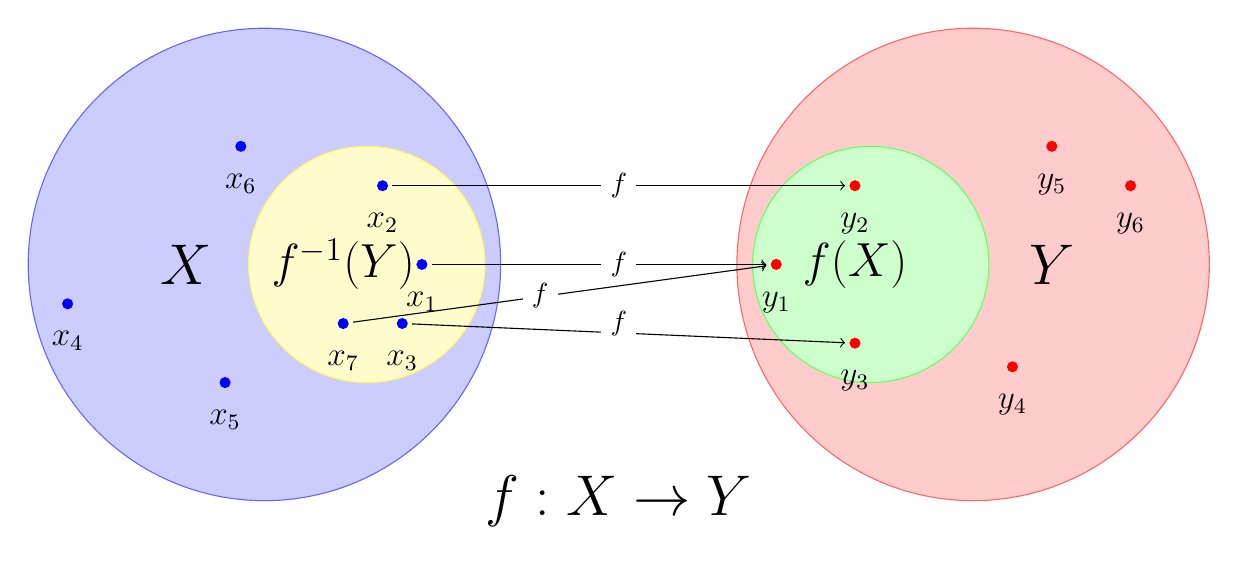
\begin{tikzpicture}[label distance=1mm]
    % draw the sets
    \filldraw[fill=blue!20, draw=blue!60] (-4.5,0) circle (3cm);
    \filldraw[fill=red!20, draw=red!60] (4.5,0) circle (3cm);
    \filldraw[fill=green!20, draw=green!60] (3.2,0) circle (1.5cm);
    \filldraw[fill=yellow!20, draw=yellow!60] (-3.2,0) circle (1.5cm);

    % the texts
    \node at (3,0) {\LARGE$f(X)$};
    \node at (-3.5,0) {\LARGE$f^{-1}(Y)$};
    \node at (-5.5,0) {\huge$X$};
    \node at (5.5,0) {\huge$Y$};
    \node at (0,-3) {\huge$f: X \to Y$};

    % the points in the sets (here I just create nodes to use them later on to position
    % the circles and the arrows
    % \node[mycirc, label=right:{$x-1$}] at (0,0) {};
    \node[label=below:{\large$x_1$}] (x1) at (-2.5,0) {};
    \node[label=below:{\large$x_2$}] (x2) at (-3,1) {};
    \node[label=below:{\large$x_3$}] (x3) at (-2.75,-0.75) {};
    \node[label=below:{\large$x_4$}] (x4) at (-7,-0.5) {};
    \node[label=below:{\large$x_5$}] (x5) at (-5,-1.5) {};
    \node[label=below:{\large$x_6$}] (x6) at (-4.8,1.5) {};
    \node[label=below:{\large$x_7$}] (x7) at (-3.5,-0.75) {};
    %
    \node[label=below:{\large$y_1$}] (y1) at (2,0) {};
    \node[label=below:{\large$y_2$}] (y2) at (3,1) {};
    \node[label=below:{\large$y_3$}] (y3) at (3,-1) {};
    \node[label=below:{\large$y_4$}] (y4) at (5,-1.3) {};
    \node[label=below:{\large$y_5$}] (y5) at (5.5,1.5) {};
    \node[label=below:{\large$y_6$}] (y6) at (6.5,1) {};

    % position the elements in the sets (at the nodes we just created)
    \fill[blue] (x1) circle (2pt);
    \fill[blue] (x2) circle (2pt);
    \fill[blue] (x3) circle (2pt);
    \fill[blue] (x4) circle (2pt);
    \fill[blue] (x5) circle (2pt);
    \fill[blue] (x6) circle (2pt);
    \fill[blue] (x7) circle (2pt);
    %
    \fill[red] (y1) circle (2pt);
    \fill[red] (y2) circle (2pt);
    \fill[red] (y3) circle (2pt);
    \fill[red] (y4) circle (2pt);
    \fill[red] (y5) circle (2pt);
    \fill[red] (y6) circle (2pt);

    % draw the arrows
    \draw[->] (x1) --  (y1);
    \node[fill=white] at (0,0) {$f$};    
    \draw[->] (x2) -- (y2);    
    \node[fill=white] at (0,1) {$f$};
    \draw[->] (x3) -- (y3);
    \node[fill=white] at (0,-0.75) {$f$};
    \draw[->] (x7) -- (y1);
    \node[fill=white] at (-1,-0.4) {$f$};
\end{tikzpicture}
\caption{Représentation de la notion d'application, d'image directe et d'image réciproque}
\label{chap3-fig:application}
\end{figure}

\section{Injection, surjection, bijection}
\label{chap3-sec:injsurbij}
%
%\begin{figure}
%  \centering
%  \includegraphics[scale=0.7, width=\textwidth]{Surjection_Injection_Bijection.png}
%  \caption[Surjection, injection et bijection]{Représentation graphique des notions de surjection, injection et bijection}
%  \label{chap3-fig:surjinjbij}
%\end{figure}
%
\subsection{Équation}
\label{chap3-subsec:equation}
\begin{defdef}
  On appelle équation, toute égalité du type
  \begin{equation}
    \Phi(a)=b,
  \end{equation}
  où~:
  \begin{itemize}
  \item \(\Phi\) est une application d'un ensemble \(A\) vers un ensemble \(B\).
  \item \(b\) est un élément de l'ensemble \(B\).
  \item \(a\) est un élément de l'ensemble \(A\), appelé \emph{inconnue} de l'équation. On appelle solution de l'équation tout élément \(a\) de l'ensemble \(A\) tel que \(\Phi(a)=b\). On note \(\mathcal{S}\) l'ensemble des solutions de l'équation
    \begin{equation}
      \mathcal{S} = \enstq{a \in A}{\Phi(a)=b}.
    \end{equation}
  \end{itemize}
\end{defdef}
\emph{Remarque \& Exemples}~: L'équation ci-dessus admet au moins une solution si et seulement si \(b \in \Phi(A)\). Les équations polynomiales de degré \(n\), les équations différentielles, les équations matricielles sont des exemples.
%
\subsection{Injection et surjection}
\label{chap3-subsec:injetsurj}
\subsubsection{Injection}
\label{chap3-subsubsec:injection}
Soient \(E\) et \(F\) des ensembles et \(f: E \longrightarrow F\) une application.
\begin{defdef}
  On dit que \(f\) est injective ou que c'est une injection si elle vérifie l'une des propriétés suivantes:
  \begin{itemize}
  \item tout élément de \(F\) admet au plus un antécédent par \(f\) dans \(E\);
  \item pour tout \(y\) de \(F\), l'équation \(f(x)=y\) admet au plus une solution dans \(E\);
  \item \(\forall (x,x') \in E^2 \quad f(x)=f(x') \implies x=x'\);
  \item \(\forall (x,x') \in E^2 \quad  x \neq x' \implies f(x) \neq f(x')\).
  \end{itemize}
  Ainsi \(f\) est non injective s'écrit
  \begin{equation}
    \exists (x,x') \in E^2 \quad x \neq x' \text{~et~} f(x) = f(x').
  \end{equation}
  La figure~\ref{chap3-fig:inj} donne une représentation graphique de la notion d'injection.
\end{defdef}
\begin{theo}
  La composée de deux applications injectives est injective.
\end{theo}
\begin{proof}
  Soient \(E,F\) et \(G\) trois ensembles et \(f:E \longrightarrow F\) et \(g: F \longrightarrow G\) deux applications injectives. Montrons que \(g \circ f\) est injective. 

Soient \(x\) et \(x'\) deux éléments de \(E\) tels que \(g \circ f(x) = g \circ f(x')\). Comme \(g\) est injective alors \(f(x)=f(x')\). Comme \(f\) est injective alors \(x=x'\). Finalement \(g \circ f\) est injective.
\end{proof}
\begin{figure}
    \centering
    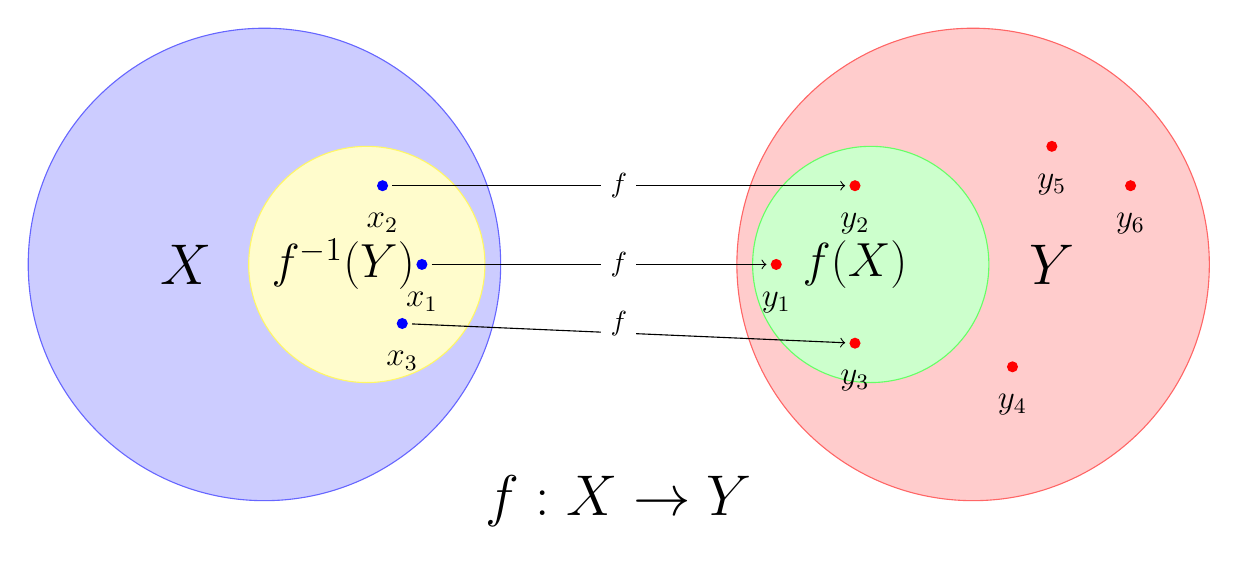
\begin{tikzpicture}[label distance=1mm]
    % draw the sets
    \filldraw[fill=blue!20, draw=blue!60] (-4.5,0) circle (3cm);
    \filldraw[fill=red!20, draw=red!60] (4.5,0) circle (3cm);
    \filldraw[fill=green!20, draw=green!60] (3.2,0) circle (1.5cm);
    \filldraw[fill=yellow!20, draw=yellow!60] (-3.2,0) circle (1.5cm);

    % the texts
    \node at (3,0) {\LARGE$f(X)$};
    \node at (-3.5,0) {\LARGE$f^{-1}(Y)$};
    \node at (-5.5,0) {\huge$X$};
    \node at (5.5,0) {\huge$Y$};
    \node at (0,-3) {\huge$f: X \to Y$};

    % the points in the sets (here I just create nodes to use them later on to position
    % the circles and the arrows
    % \node[mycirc, label=right:{$x-1$}] at (0,0) {};
    \node[label=below:{\large$x_1$}] (x1) at (-2.5,0) {};
    \node[label=below:{\large$x_2$}] (x2) at (-3,1) {};
    \node[label=below:{\large$x_3$}] (x3) at (-2.75,-0.75) {};
    %\node[label=below:{\large$x_4$}] (x4) at (-7,-0.5) {};
    %\node[label=below:{\large$x_5$}] (x5) at (-5,-1.5) {};
    %\node[label=below:{\large$x_6$}] (x6) at (-4.8,1.5) {};
    %\node[label=below:{\large$x_7$}] (x7) at (-3.5,-0.75) {};
    %
    \node[label=below:{\large$y_1$}] (y1) at (2,0) {};
    \node[label=below:{\large$y_2$}] (y2) at (3,1) {};
    \node[label=below:{\large$y_3$}] (y3) at (3,-1) {};
    \node[label=below:{\large$y_4$}] (y4) at (5,-1.3) {};
    \node[label=below:{\large$y_5$}] (y5) at (5.5,1.5) {};
    \node[label=below:{\large$y_6$}] (y6) at (6.5,1) {};

    % position the elements in the sets (at the nodes we just created)
    \fill[blue] (x1) circle (2pt);
    \fill[blue] (x2) circle (2pt);
    \fill[blue] (x3) circle (2pt);
    %\fill[blue] (x4) circle (2pt);
    %\fill[blue] (x5) circle (2pt);
    %\fill[blue] (x6) circle (2pt);
    %\fill[blue] (x7) circle (2pt);
    %
    \fill[red] (y1) circle (2pt);
    \fill[red] (y2) circle (2pt);
    \fill[red] (y3) circle (2pt);
    \fill[red] (y4) circle (2pt);
    \fill[red] (y5) circle (2pt);
    \fill[red] (y6) circle (2pt);

    % draw the arrows
    \draw[->] (x1) --  (y1);
    \node[fill=white] at (0,0) {$f$};    
    \draw[->] (x2) -- (y2);    
    \node[fill=white] at (0,1) {$f$};
    \draw[->] (x3) -- (y3);
    \node[fill=white] at (0,-0.75) {$f$};
    %\draw[->] (x7) -- (y1);
    %\node[fill=white] at (-1,-0.4) {$f$};
\end{tikzpicture}
    \caption[Injection]{Représentation graphique d'une injection}
    \label{chap3-fig:inj}
\end{figure}
\subsubsection{Surjection}
\label{chap3-subsubsec:surjection}
\begin{defdef}
  On dit que f est une surjection, ou qu'elle est surjective si elle vérifie l'une des propriétés suivantes~:
  \begin{itemize}
  \item tout élément de \(F\) admet au moins un antécédent par \(f\) dans \(E\);
  \item pour tout \(y\) de \(F\), l'équation \(f(x)=y\) admet au moins une solution dans \(E\);
  \item \(\forall y \in F \ \exists x \in E \quad y=f(x)\);
  \end{itemize}
  Ainsi \(f\) est non surjective s'écrit
  \begin{equation}
    \exists y \in F \ \forall x \in E \quad y \neq f(x).
  \end{equation}
  La figure~\ref{chap3-fig:surj} donne une représentation graphique de la notion de surjection.
\end{defdef}
\begin{prop}
  Une application \(f:E \longrightarrow F\) est surjective si et seulement si \(f(E)=F\).
\end{prop}
\begin{proof}
    Par définition tout élément de \(F\) admet au moins un antécédent par \(f\) dans \(E\), ce qui équivaut à \(F \subset f(E)\) et l'autre inclusion est évidente par définition des applications \(f(E) \subset F\).
\end{proof}
\begin{theo}
  La composée de deux applications surjectives est surjective.
\end{theo}
\begin{proof}
  Soient \(f:E \longrightarrow F\) et \(g:F \longrightarrow G\) deux surjections, montrons que \(g \circ f: E \longrightarrow G\) est surjective. 

  Soit \(z \in G\), puisque \(g\) est surjective alors il existe \(y \in F\) tel que \(z=g(y)\). Puisque \(y \in F\) et que \(f\) est surjective alors il existe \(x\) tel que \(y=f(x)\). Finalement, on a montré qu'il existe \(x \in E\) tel que \(z=g(y)=g(f(x))= g \circ f(x)\).
\end{proof}
\begin{figure}
    \centering
   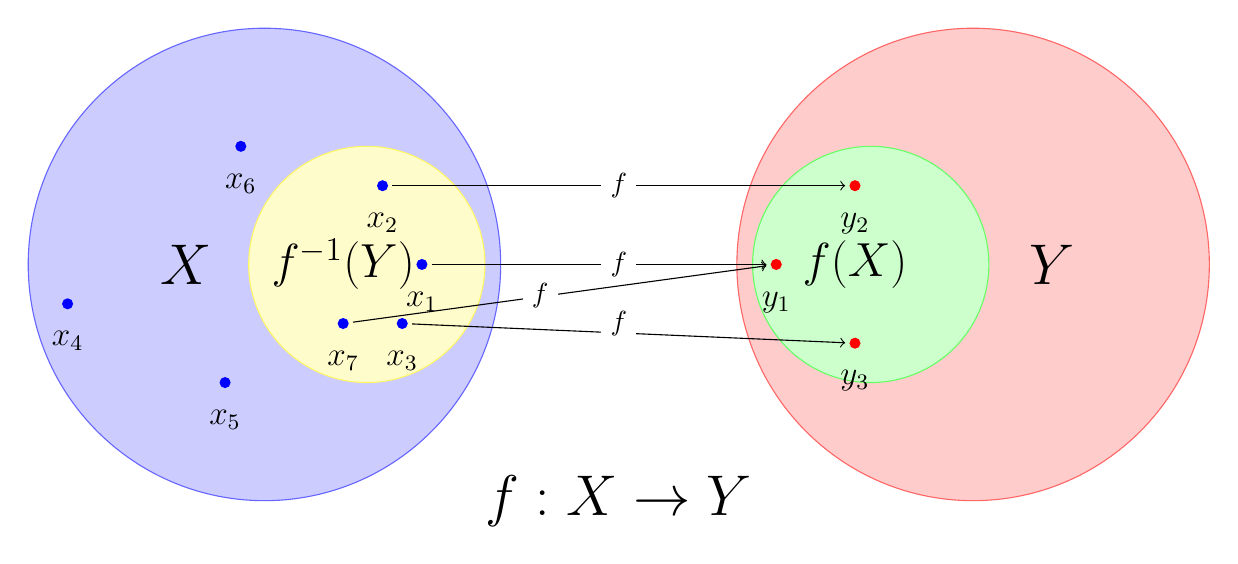
\begin{tikzpicture}[label distance=1mm]
    % draw the sets
    \filldraw[fill=blue!20, draw=blue!60] (-4.5,0) circle (3cm);
    \filldraw[fill=red!20, draw=red!60] (4.5,0) circle (3cm);
    \filldraw[fill=green!20, draw=green!60] (3.2,0) circle (1.5cm);
    \filldraw[fill=yellow!20, draw=yellow!60] (-3.2,0) circle (1.5cm);

    % the texts
    \node at (3,0) {\LARGE$f(X)$};
    \node at (-3.5,0) {\LARGE$f^{-1}(Y)$};
    \node at (-5.5,0) {\huge$X$};
    \node at (5.5,0) {\huge$Y$};
    \node at (0,-3) {\huge$f: X \to Y$};

    % the points in the sets (here I just create nodes to use them later on to position
    % the circles and the arrows
    % \node[mycirc, label=right:{$x-1$}] at (0,0) {};
    \node[label=below:{\large$x_1$}] (x1) at (-2.5,0) {};
    \node[label=below:{\large$x_2$}] (x2) at (-3,1) {};
    \node[label=below:{\large$x_3$}] (x3) at (-2.75,-0.75) {};
    \node[label=below:{\large$x_4$}] (x4) at (-7,-0.5) {};
    \node[label=below:{\large$x_5$}] (x5) at (-5,-1.5) {};
    \node[label=below:{\large$x_6$}] (x6) at (-4.8,1.5) {};
    \node[label=below:{\large$x_7$}] (x7) at (-3.5,-0.75) {};
    %
    \node[label=below:{\large$y_1$}] (y1) at (2,0) {};
    \node[label=below:{\large$y_2$}] (y2) at (3,1) {};
    \node[label=below:{\large$y_3$}] (y3) at (3,-1) {};
    %\node[label=below:{\large$y_4$}] (y4) at (5,-1.3) {};
    %\node[label=below:{\large$y_5$}] (y5) at (5.5,1.5) {};
    %\node[label=below:{\large$y_6$}] (y6) at (6.5,1) {};

    % position the elements in the sets (at the nodes we just created)
    \fill[blue] (x1) circle (2pt);
    \fill[blue] (x2) circle (2pt);
    \fill[blue] (x3) circle (2pt);
    \fill[blue] (x4) circle (2pt);
    \fill[blue] (x5) circle (2pt);
    \fill[blue] (x6) circle (2pt);
    \fill[blue] (x7) circle (2pt);
    %
    \fill[red] (y1) circle (2pt);
    \fill[red] (y2) circle (2pt);
    \fill[red] (y3) circle (2pt);
    %\fill[red] (y4) circle (2pt);
    %\fill[red] (y5) circle (2pt);
    %\fill[red] (y6) circle (2pt);

    % draw the arrows
    \draw[->] (x1) --  (y1);
    \node[fill=white] at (0,0) {$f$};    
    \draw[->] (x2) -- (y2);    
    \node[fill=white] at (0,1) {$f$};
    \draw[->] (x3) -- (y3);
    \node[fill=white] at (0,-0.75) {$f$};
    \draw[->] (x7) -- (y1);
    \node[fill=white] at (-1,-0.4) {$f$};
    \end{tikzpicture} 
\caption[Surjection]{Représentation graphique d'une surjection}
\label{chap3-fig:surj}
\end{figure}
\subsection{Bijection}
\label{chap3-subsubsec:bijection}
Soient \(E\) et \(F\) deux ensemble et \(f:E \longrightarrow F\) une application.
\begin{defdef}
  On dit que \(f\) est bijective lorsqu'elle vérifie une des propriétés suivantes équivalentes
  \begin{itemize}
  \item Tout élément de \(F\) admet un et un seul antécédent par \(f\) dans \(E\);
  \item pour tout \(y \in F\) l'équation \(y=f(x)\) admet exactement une solution dans \(E\);
  \item \(\forall y \in F \ \exists! x \in E \quad f(x)=y\);
  \item \(f\) est injective et surjective.
  \end{itemize}
La figure~\ref{chap3-fig:bij} donne une représentation graphique de la notion de bijection.
\end{defdef}
%
Soit \(f=(E,F,\Gamma)\) une bijection, on pose 
\begin{equation}
\Gamma^{-1}=\enstq{(y,x) \in F \times E}{(x,y) \in \Gamma}
\end{equation}
pour tout \((y,x) \in F \times E\), on a les équivalences suivantes
\begin{equation}
  (y,x) \in \Gamma^{-1} \iff (x,y) \in \Gamma \iff y=f(x).
\end{equation}

Pour tout \(y \in F\) il existe un unique \(x \in E\) tel que \(y=f(x)\) ---~définition de la bijection~--- c'est-à-dire un unique \(x \in E\) tel que \((y,x) \in \Gamma^{-1}\). L'application \((F,E,\Gamma^{-1})\) est l'application réciproque de \(f\) et on la note \(f^{-1}\).
%
\begin{prop} Soit une bijection \(f : E \longrightarrow F\). Alors \(f^{-1} : F \longrightarrow E\) est une bijection et
  \begin{gather}
    f^{-1} \circ f =\Id_E; \\
    f \circ f^{-1}=\Id_F.
  \end{gather}
\end{prop}
\begin{proof}
Soit \((x,y) \in E \times F\) tels que \(x=f^{-1}(y) \iff y=f(x)\). Pour tous élément \(x\) de \(E\), il existe un unique \(y\) dans \(F\) tel que \(x=f^{-1}(y)\). Donc \(f^{-1}\) est une bijection.
\end{proof}
\begin{figure}
    \centering
    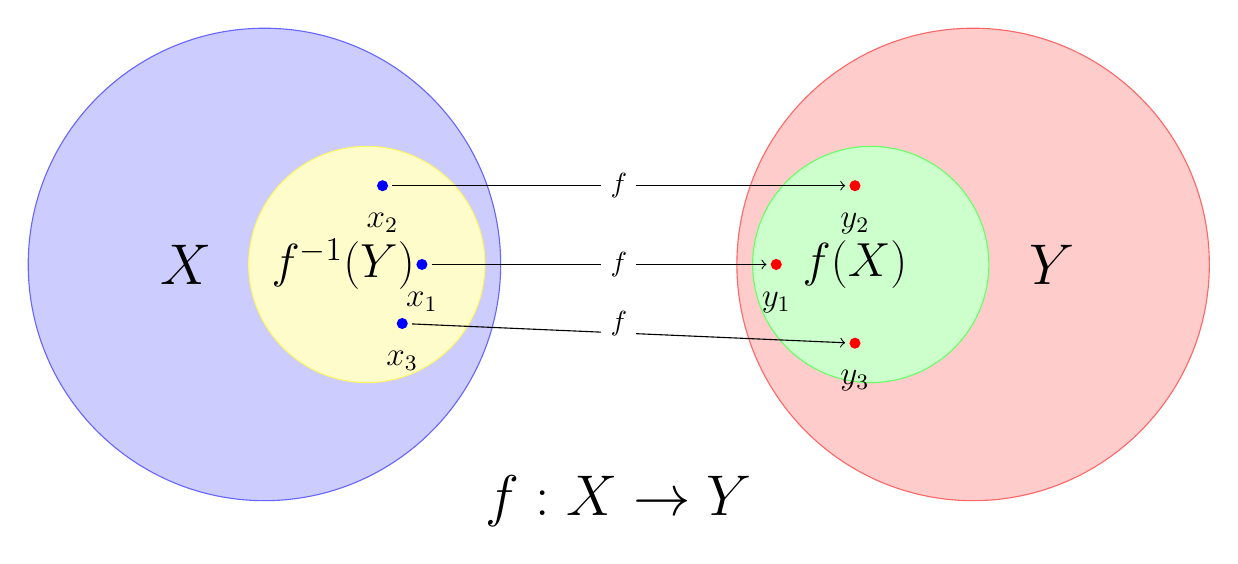
\begin{tikzpicture}[label distance=1mm]
    % draw the sets
    \filldraw[fill=blue!20, draw=blue!60] (-4.5,0) circle (3cm);
    \filldraw[fill=red!20, draw=red!60] (4.5,0) circle (3cm);
    \filldraw[fill=green!20, draw=green!60] (3.2,0) circle (1.5cm);
    \filldraw[fill=yellow!20, draw=yellow!60] (-3.2,0) circle (1.5cm);

    % the texts
    \node at (3,0) {\LARGE$f(X)$};
    \node at (-3.5,0) {\LARGE$f^{-1}(Y)$};
    \node at (-5.5,0) {\huge$X$};
    \node at (5.5,0) {\huge$Y$};
    \node at (0,-3) {\huge$f: X \to Y$};

    % the points in the sets (here I just create nodes to use them later on to position
    % the circles and the arrows
    % \node[mycirc, label=right:{$x-1$}] at (0,0) {};
    \node[label=below:{\large$x_1$}] (x1) at (-2.5,0) {};
    \node[label=below:{\large$x_2$}] (x2) at (-3,1) {};
    \node[label=below:{\large$x_3$}] (x3) at (-2.75,-0.75) {};
    %\node[label=below:{\large$x_4$}] (x4) at (-7,-0.5) {};
    %\node[label=below:{\large$x_5$}] (x5) at (-5,-1.5) {};
    %\node[label=below:{\large$x_6$}] (x6) at (-4.8,1.5) {};
    %\node[label=below:{\large$x_7$}] (x7) at (-3.5,-0.75) {};
    %
    \node[label=below:{\large$y_1$}] (y1) at (2,0) {};
    \node[label=below:{\large$y_2$}] (y2) at (3,1) {};
    \node[label=below:{\large$y_3$}] (y3) at (3,-1) {};
    %\node[label=below:{\large$y_4$}] (y4) at (5,-1.3) {};
    %\node[label=below:{\large$y_5$}] (y5) at (5.5,1.5) {};
    %\node[label=below:{\large$y_6$}] (y6) at (6.5,1) {};

    % position the elements in the sets (at the nodes we just created)
    \fill[blue] (x1) circle (2pt);
    \fill[blue] (x2) circle (2pt);
    \fill[blue] (x3) circle (2pt);
    %\fill[blue] (x4) circle (2pt);
    %\fill[blue] (x5) circle (2pt);
    %\fill[blue] (x6) circle (2pt);
    %\fill[blue] (x7) circle (2pt);
    %
    \fill[red] (y1) circle (2pt);
    \fill[red] (y2) circle (2pt);
    \fill[red] (y3) circle (2pt);
    %\fill[red] (y4) circle (2pt);
    %\fill[red] (y5) circle (2pt);
    %\fill[red] (y6) circle (2pt);

    % draw the arrows
    \draw[->] (x1) --  (y1);
    \node[fill=white] at (0,0) {$f$};    
    \draw[->] (x2) -- (y2);    
    \node[fill=white] at (0,1) {$f$};
    \draw[->] (x3) -- (y3);
    \node[fill=white] at (0,-0.75) {$f$};
    %\draw[->] (x7) -- (y1);
    %\node[fill=white] at (-1,-0.4) {$f$};
    \end{tikzpicture}
    \caption[Bijection]{Représentation graphique d'une bijection}
    \label{chap3-fig:bij}
\end{figure}

\begin{theo}[Caractérisation des bijections]
Soient \(E\) et \(F\) des ensembles et \(f:E \longrightarrow F\) une application. L'application \(f\) est une bijection si et seulement s'il existe une application \(g:F \longrightarrow E\) telle que \(g \circ f = \Id_E\) et \(f \circ g = \Id_F\). Auquel cas \(g\) est unique et \(g=f^{-1}\).
\end{theo}
\begin{proof}
  Supposons l'existence d'une application \(g:F \longrightarrow E\) telle que \(g \circ f = \Id_E\) et \(f \circ g = \Id_F\). Montrons que \(f\) est injective et surjective.
  \begin{itemize}
  \item Soient \(x\) et \(x'\) dans \(E\) tels que \(f(x)=f(x')\) alors \(g \circ f(x) = g \circ f(x')\) donc \(x=x'\). \(f\) est donc injective.
  \item Soit \(y \in F\) alors \(y=\Id_F(y)=f(g(y))\) si on pose \(x=g(y) \in E\) alors \(y=f(x)\). On a montré qu'il existe \(x \in E\) tel que y=f(x), donc \(f\) est surjective.
  \end{itemize}
  On en conclus que \(f\) est bijective.
\end{proof}
%
\begin{prop}
  Soient \(E,F,G\) trois ensembles et deux applications \(f:E \longrightarrow F\) et \(g:F \longrightarrow G\) alors si \(g \circ f\) est injective (respectivement surjective) alors \(f\) est injective (respectivement surjective).
\end{prop}
\begin{proof}
  \begin{itemize}
  \item Soient \(x\) et \(x'\) dans \(E\) tels que \(f(x)=f(x')\) alors \(g \circ f(x) = g \circ f(x')\) et puisque \(g \circ f\) est injective donc \(x=x'\) donc \(f\) est injective.
  \item Soit \(y\) un élément de \(F\), \(f \circ g\) est surjective donc il existe \(x \in F\) tel que \(y=f \circ g(x)=f(g(x))\) donc \(f\) est surjective.
  \end{itemize}
\end{proof}
%
\begin{prop}
La composée de deux applications bijectives est bijective.
\end{prop}
\begin{proof}
La composée de deux applications surjectives est surjective et la composée de deux applications injectives est injective donc la composée de deux applications bijectives est bijective.
\end{proof}
%
\begin{defdef}
\begin{enumerate}
\item On appelle permutation de \(E\) toute bijection de \(E\) dans \(E\);
\item on appelle involution de \(E\) toute application \(f: E \longrightarrow E\) telle que \(f \circ f=\Id_E\). Une involution de \(E\) est une permutation de \(E\) telle que \(f=f^{-1}\).
\end{enumerate}
\end{defdef}
%
\emph{Remarques}~:
\begin{enumerate}
\item Si \(f\) est une involution alors les courbes représentatives de \(f\) et \(f^{-1}\) sont symétriques par rapport à la première bissectrice;
\item soit \(f\) une application bijective de \(E\) dans \(F\) et \(B\) une partie de \(F\). On dispose de \(A_1=f^{-1}(B)\) l'image réciproque de \(B\) par rapport à \(f\), \(A_2=f^{-1}(B)\) l'image directe de \(B\) par \(f^{-1}\). On a aussi \(A_1=A_2\).
\end{enumerate}
%
\section{Relations}
\label{chap3-sec:relations}
\subsection{Relations binaires}
\label{chap3-subsec:relationbinaire}
\begin{defdef}
On appelle correspondance entre éléments d'un ensemble \(E\) et éléments d'un ensemble \(F\) tout triplet \((E,F,G)\) où \(G\) est une partie de \(E \times F\). \(E\) est appelé ensemble de départ, \(F\) ensemble d'arrivée et \(G\) le graphe de la correspondance. Dans le cas où \(E=F\), on parle de relation binaire sur l'ensemble \(E\).
\end{defdef}
%
\emph{Notation}~: Si \(\RelBin=(E,E,G)\) est une relation binaire sur \(E\), au lieu de noter \((x,y) \in G\). On écrira \(x\RelBin{}y\) et on dira que les éléments de \(x\) et \(y\), pris dans cette ordre, vérifient la relation \(\RelBin\).
\begin{defdef}
On peut définir des qualités éventuelles d'une relation binaire. Soit \(E\) un ensemble et \(\RelBin{}\) une relation binaire sur \(E\), on définit~:
\begin{enumerate}
\item \(\RelBin{}\) est réflexive si \(\forall x \in E \quad x\RelBin{}x\);
\item \(\RelBin{}\) est symétrique si \(\forall (x,y) \in E^2 \quad x\RelBin{}y \implies y\RelBin{}x\);
\item \(\RelBin{}\) est antisymétrique si \(\forall (x,y) \in E^2 \quad x\RelBin{}y \text{~et~} y\RelBin{}x \implies y=x\);
\item \(\RelBin{}\) est transitive si \(\forall (x,y,z) \in E^3 \quad x\RelBin{}y \text{~et~} y\RelBin{}z \implies x\RelBin{}z\).
\end{enumerate}
\end{defdef}
%
\subsection{Relations d'ordre}
\label{chap3-subsec:relationdordre}
\subsubsection{Définition et exemples}
\label{chap3-subsubsec:relationordredef}
\begin{defdef}
On appelle relation d'ordre sur \(E\) toute relation binaire sur \(E\) qui est réflexive, antisymétrique et transitive. Un ensemble muni d'une relation d'ordre est appelé un ensemble ordonné. On note souvent \(\prec\) les relations d'ordre, on réserve la notation \(\leqslant\) à l'ordre usuel, sur les ensembles de nombres.
\end{defdef}

\emph{Exemples}~: les relations d'ordres usuelles sur \(\R\), \(\Z\), \(\Q\) et \(\N\); La relation d'ordre strict sur \(\R\) n'est pas une relation d'ordre car elle n'est pas réflexive. La relation de divisibilité est une relation d'ordre sur \(\N\). La relation d'inclusion sur l'ensemble \(\mathfrak{P}(E)\) est une relation d'ordre.
%
\subsubsection{Éléments comparables - Ordre total}
\label{chap3-subsubsec:ordretotal}
\begin{defdef}
Soit \((E, \prec)\) un ensemble ordonné. Deux éléments \(x\) et \(y\) de \(E\) sont dits comparables par la relation d'ordre \(\prec\) si et seulement si l'une au moins des relations \(x \prec y\) ou \(y \prec x\) est vérifiée.
\end{defdef}
\begin{defdef}
On dit que \((E, \prec)\) est un ensemble totalement ordonné ou encore que l'ordre \(\prec\) est total si et seulement si pour tous les éléments \(x\) et \(y\) pris dans \(E\), \(x\) et \(y\) sont comparables par \(\prec\). Sinon on dit que \((E,\prec)\) est partiellement ordonné ou encore que l'ordre \(\prec\) est partiel.
\end{defdef}
%
\subsubsection{Éléments remarquables d'un ensemble ordonné}
\label{chap3-subsubsec:elementremarquables}
Soit \((E,\prec)\) un ensemble ordonné et \(A\) une partie de \(E\).
\begin{defdef}[Partie majorée, minorée, bornée]
\begin{enumerate}
\item Un élément \(M\) de \(E\) est appelé un majorant de la partie \(A\) dans \(E\) si et seulement si \(\forall a \in A \quad a \prec M\), on dit que la partie \(A\) est majorée dans \(E\) si et seulement si elle admet un majorant dans \(E\);
\item un élément \(m\) de \(E\) est appelé un minorant de la partie \(A\) dans \(E\) si et seulement si \(\forall a \in A \quad m \prec a\), on dit que la partie \(A\) est minorée dans \(E\) si et seulement si elle admet un minorant dans \(E\);
\item une partie \(A\) de \(E\) est dite bornée dans \(E\) lorsqu'elle est à la fois majorée dans \(E\) et minorée dans \(E\).
\end{enumerate}
Il est important de préciser dans quel ensemble la partie est majorée et minorée.
\end{defdef}
%
\begin{defdef}[plus petit et plus grand élément]
\begin{enumerate}
\item On appelle un plus petit élément de la partie \(A\) tout élément de \(A\) qui minore \(A\) dans \(E\), si \(A\) admet un plus petit élément celui-ci est unique et on l'appelle \emph{le} plus petit élément de \(A\);
\item on appelle un plus grand élément de la partie \(A\) tout élément de \(A\) qui majore \(A\) dans \(E\), si \(A\) admet un plus grand élément celui-ci est unique et on l'appelle \emph{le} plus grand élément de \(A\).
\end{enumerate}
\end{defdef}
\begin{proof}[Unicité]
\begin{enumerate}
\item Si \(a\) et \(b\) sont les plus petits éléments de \(A\) alors comme \(a\) est un minorant \(a \prec b\) et puisque \(b\) est un minorant \(b \prec a\) et comme \(\prec\) est antisymétrique on a forcément \(a=b\).
\item On démontre l'unicité du plus grand élément de la même manière.
\end{enumerate}
\end{proof}
%
\emph{Exemples}~:
\begin{enumerate}
\item Dans \((\mathfrak{P}(E), \subset)\) \(\emptyset\) est le plus petit élément et \(E\) est le plus grand.
\item Dans \((\N,|)\), avec \(|\) la relation de divisibilité, \(1\) est le plus petit élément et \(0\) est le plus grand.
\end{enumerate}
%
\begin{defdef}[Borne supérieure et borne inférieure]
\begin{enumerate}
\item La borne supérieure de la partie \(A\) dans \(E\) est le plus petit élément, s'il existe, de l'ensemble des majorants de la partie \(A\) dans \(E\);
\item la borne inférieure de la partie \(A\) dans \(E\) est le plus grand élément, s'il existe, de l'ensemble des minorants de la partie \(A\) dans \(E\).
\end{enumerate}
\end{defdef}
%
\subsection{Relation d'équivalence}
\label{chap3-subsec:relationequivalence}
\begin{defdef}
On appelle relation d'équivalence sur \(E\) toute relation binaire qui est réflexive, symétrique et transitive
\end{defdef}
On note généralement \(\sim\) les relations d'équivalences. Si \(x \sim y\), on dit que \(x\) est équivalent à \(y\), ou encore, compte tenu de la symétrie, que \(x\) et \(y\) sont équivalents. Par exemple, on peut citer l'égalité, la congruence, la similitude de matrice ou l'équivalence de matrices.
%
\section{Familles}
\label{chap3-sec:familles}
\subsection{Notion de famille}
\label{chap3-subsec:notionfamille}
\begin{defdef}
Soient \(E\) et \(I\) des ensembles quelconques. On appelle famille d'éléments de \(E\) indexée par \(I\) toute application \(\mathcal{U} : I \longrightarrow E\), on notera \(\mathcal{U}=(u_i)_{i \in I}\).
\end{defdef}
%
On dit que \(I\) est l'ensemble des indices de la famille \(\mathcal{U}\). On notera \(E^I\) l'ensemble des familles de \(E\) indexées par \(I\). Par exemple, si l'ensemble des indices est \(\N\) alors \(E^{\N}\) est l'ensemble des suites à valeur dans \(E\). Si \(I\) est un ensemble fini, on identifie les familles indexées par \(I\) à des listes de longueur Cardinal(\(I\)).
%
\subsection{Familles de parties d'un ensemble}
\label{chap3-subsec:familledeparties}
Soit \(E\) un ensemble.
\begin{defdef}
  Soit \((A_i)_{i \in I}\) une famille de parties de \(E\), on définit
  \begin{enumerate}
  \item L'intersection de la famille \((A_i)_{i \in I}\)  \(\bigcap\limits_{i \in I} A_i = \enstq{x \in E}{\forall i \in I \quad x \in A_i}\);
  \item La réunion de la famille \((A_i)_{i \in I}\)  \(\bigcup\limits_{i \in I} A_i = \enstq{x \in E}{\exists i \in I \quad x \in A_i}\).
  \end{enumerate}
\end{defdef}
Ainsi, l'intersection est l'ensemble des éléments de \(E\) qui appartiennent à chacun des \(A_i\) et la réunion est l'ensemble des éléments de \(E\) qui appartiennent à au moins un des \(A_i\).

\emph{Remarques}~:
\begin{enumerate}
\item Si \(I=\{1,2\}\), on retrouve la définition de l'intersection et de la réunion de deux parties de \(A\).
\item Si \(I \neq \emptyset\), il existe \(i_0 \in I\) tel que \(\bigcap\limits_{i \in I} A_i \subset A_{i_0} \subset \bigcup\limits_{i \in I} A_i\).
\item Si \(I = \emptyset\) alors \(\bigcap\limits_{i \in I} A_i =E \quad \bigcup\limits_{i \in I} A_i=\emptyset\).
\end{enumerate}
%
\subsubsection{Formulaire}
\label{chap3-subsubsec:formulaireensemble}
\paragraph{Lois de Morgan}
\label{chap3-par:morgan}
\begin{align}
  E \setminus \bigcup\limits_{i \in I} A_i &= \bigcap\limits_{i \in I} E \setminus A_i;\\
  E \setminus \bigcap\limits_{i \in I} A_i &= \bigcup\limits_{i \in I} E \setminus A_i.
\end{align}
\paragraph{Images directes}
\label{chap3-par:imagedir}
Soit une application \(f \in F^E\) une application si \((A_i)_{i \in I}\) est une famille de parties de \(E\), on dispose de \((f(A_i))_{i \in I}\) familles de parties de \(F\) et on a 
\begin{align}
  f \left(\bigcap\limits_{i \in I} A_i\right) &\subset \bigcap\limits_{i \in I} f(A_i);\\
  f \left(\bigcup\limits_{i \in I} A_i\right) &= \bigcap\limits_{i \in I} f(A_i).
\end{align}
\paragraph{Images réciproques}
\label{chap3-par:imagerec}
Si on dispose d'une famille de parties de \(F\) \((B_i)_{i \in I}\) alors on peut utiliser la famille \((f^{-1}(B_i))_{i \in I}\) de parties de \(E\) et on a 
\begin{align}
  f^{-1} \left(\bigcap\limits_{i \in I} B_i\right) &= \bigcap\limits_{i \in I} f^{-1}(B_i);\\
  f^{-1} \left(\bigcup\limits_{i \in I} B_i\right) &= \bigcap\limits_{i \in I} f^{-1}(B_i).
\end{align}
\subsection{Opérations sur des familles de complexes indexées par un ensemble fini}
\label{chap3-subsec:operationsfamilles}
On suppose que \(I=(i_k)_{k \in  \intervalleentier{1}{n}}\). On note 
\begin{align}
  \sum_{i \in I} u_i &= u_{i_1} +u_{i_2} +u_{i_3} + \dotsb +u_{i_n}; \\
  \prod_{i \in I} u_i &= u_{i_1} \times u_{i_2} \times u_{i_3} \times \dotsm \times u_{i_n}. 
\end{align}
Si \(I=\emptyset\) alors \(\sum_{i \in I} u_i=0\) et \(\prod_{i \in I} u_i=1\) par convention.
\cleardoublepage
\section{Exercices --- Ensembles, applications et relations binaires}
\begin{exercice}
    Pour chacun des ensembles \(E\) suivants, déterminer les éléments de l'ensemble \(\Part(E)\) des parties de \(E\), puis les éléments de l'ensemble \(\Part(\Part(E))\).
    \begin{enumerate}
        \item \(E=\emptyset\);
        \item \(E\) est un singleton \(\{a\}\);
        \item \(E\) est une paire \(\{a, b\}\).
    \end{enumerate}
\end{exercice}
\begin{exercice}
    Soient \(E\) un ensemble quelconque et \(A\) et \(B\) deux parties de \(E\). Démontrer les équivalences suivantes~:
    \begin{enumerate}
        \item \(A \cap B = A \iff A \subset B \);
        \item \(A \cup B = A \iff B \subset A \);
        \item \(A \cup B = A \cap B \iff A = B \).
    \end{enumerate}
\end{exercice}
\begin{exercice}[Résolution dans \(\Part(E)\) des équations \(X \cup Y=A\) et \(X \cap Y=A\)]
    Soient \(E\) un ensemble et \(A\) une partie de \(E\).
    \begin{enumerate}
        \item Montrer que \((X,Y)\in\Part(E)^2\) est solution de \(X \cup Y=A\) si et seulement s'il existe \((U, V) \in \Part(E)^2\) tel que \[X=A\cup(U\cap \complement V) \ Y=A\cup(\complement U \cap V)\].
        \item Résoudre dans \(\Part(E)^2\) l'équation \(X \cup Y = A\).
    \end{enumerate}
\end{exercice}
\begin{exercice}[Caractérisation des injections]
    Soient \(E\) et \(F\) deux ensembles et une application \(f \in F^E\).
    \begin{enumerate}
        \item Montrer que si \(f\) est injective alors pour tout couple \((A,B) \in \Part(E)^2, f(A\cap B) = f(A) \cap f(B)\). Prouver que cette égalité peut avoir lieu pour une application \(f\) non injective.
        \item Établir que \(f\) est injective si et seulement si \(\forall (A,B) \in \Part(E)^2, f(A\cap B) = f(A) \cap f(B)\).
    \end{enumerate}
\end{exercice}
\begin{exercice}
    \begin{enumerate}
        \item Soit \(f : \C^* \longrightarrow \C\) définie par \(f(z)=z+1/z\). L'application \(f\) est-elle surjective ? Est-elle injective ?
        \item Soit \(g : \R^* \longrightarrow \R\) définie par \(g(x)=x+1/x\). L'application \(g\) est-elle surjective ? Est-elle injective ?
        \item Peut on trouver des sous-ensembles \(A\) et \(B\) de \(\R^*\) et \(\R\) tels que la restriction \(h\) de \(g\) à \(A\) au départ et à \(B\) à l'arrivée soit bijective ?
    \end{enumerate}
\end{exercice}
\begin{exercice}
    Soit \(\fonctionL{f}{\R}{\R}{x}{-x^2+3x+1}\). Déterminer \(f(\R)\), \(f(\intervalleff{0}{5})\), \(f^{-1}(\intervalleff{0}{1})\), \(f^{-1}(\intervalleff{1}{4})\) et \(f(f^{-1}(\intervalleff{1}{4}))\).
\end{exercice}
\begin{exercice}
    Soit \(E\) un ensemble. Démontrer qu'il n'existe pas de surjection \(\varphi\) de \(E\) sur \(\Part(E)\). On pourra raisonner par l'absurde et introduire l'ensemble \(A=\enstq{a \in E}{a \not\in \varphi(a)}\).
\end{exercice}
\begin{exercice}
    Soient \(f : E \longrightarrow F, g : F \longrightarrow G, h : G \longrightarrow E\) trois applications telles que \(h \circ g \circ f\) et \(g \circ f \circ h\) sont injectives et \(f \circ h \circ g\) est surjective. Montrer que \(f, g, h\) sont bijectives.
\end{exercice}
\begin{exercice}[Conjugaison]
    Soient \(E\) un ensemble et \(f : E \longmapsto E\) bijective. La conjugaison par \(f\) est l'application \(\Phi_f : E^E \longmapsto E^E\) définie par
    \begin{equation}
        \forall \varphi \in E^E \quad \Phi_f(\varphi) = f \circ \varphi \circ f^{-1}.
    \end{equation}
    \begin{enumerate}
        \item Montrer que \(\Phi_f\) est une bijection de \(E^E\).
        \item Si \(g : E \longmapsto E\) est une autre application bijective, simplifier \(\Phi_f \circ \Phi_g\).
        \item Pour toutes \(\varphi, \psi \in E^E\), simplifier  \(\Phi_f(\varphi) \circ \Phi_g(\psi)\).
        \item Montrer que l'image par \(\Phi_f\) d'une application injective (respectivement surjective) est une application injective (respectivement surjective).
        \item Si \(\varphi\) est bijective, expliciter \((\Phi_f(\varphi))^{-1}\).
    \end{enumerate}
\end{exercice}
\begin{exercice}[Factorisation d'une application]
    \begin{enumerate}
        \item Soient \(f : F \longmapsto E\) et \(g : G \longmapsto E\) deux applications. Montrer qu'il existe une application \(h : G \longmapsto F\) telle que \(g = f \circ h\) si et seulement si \(g(G) \subset f(F)\). A quelle condition \(h\) est-elle unique ?
        \item Soient \(f : E \longmapsto F\) et \(g : E \longmapsto F\) deux applications. Montrer qu'il existe une application \(h : F \longmapsto G\) telle que \(g = f \circ h\) si et seulement si 
            \begin{equation}
                \forall x,y \in E \qquad f(x)=f(y) \implies g(x)=g(y).
            \end{equation}
        A quelle condition \(h\) est elle unique ?
    \end{enumerate}
\end{exercice}
\begin{exercice}
    Soient \(E\) et \(F\) deux ensembles, \(f : E \longmapsto F\) une application et \(G\) un ensemble ayant au moins deux éléments. On construit deux nouvelles applications~:
    \begin{equation}
        \fonction{f_{*}}{E^G}{F^G}{\varphi}{f \circ \varphi} \quad \fonction{f^{*}}{G^F}{G^E}{\varphi}{\varphi \circ f}
    \end{equation}
    Montrer que~:
    \begin{enumerate}
        \item \(f\) est injective si et seulement si \(f_{*}\) est injective si et seulement si \(f^{*}\) est surjective ;
        \item \(f\) est surjective si et seulement si \(f_{*}\) est surjective si et seulement si \(f^{*}\) est injective.
    \end{enumerate}
\end{exercice}
\begin{exercice}[Caractérisation des bijections]
    Soient \(E\) et \(F\) deux ensembles.
    \begin{enumerate}
        \item Montrer que pour tout \(B \in \Part(F)\),
            \begin{equation}
                f^{-1}(F\setminus B) = E \setminus f^{-1}(B)
            \end{equation}
        \item Montrer que \(f\) est bijective si et seulement si~:
            \begin{equation}
                \forall A \in \Part(E) \quad f(E\setminus A) = F\setminus f(A)
            \end{equation}
    \end{enumerate}
\end{exercice}
\begin{exercice}
    Soit \(f : E \longmapsto F\). Pour tout entier naturel non nul \(n\), on note \(f^n = \underbrace{f \circ f \circ \cdots \circ f}_{n \textrm{ fois}}\) et on pose \(f^0=\Id_E\). Soient \(A\) une partie de \(E\), \(A_n=f^{n}(A)\) et \(B = \bigcup_{n\in \N} A_n\).
    \begin{enumerate}
        \item Montrer que \(f(B) \subset B\).
        \item Montrer que \(B\) est la plus petite partie de \(E\) stable par \(f\) contenant \(A\) (c'est-à-dire la plus petite partie \(C\) de \(E\) telle que \(f(C) \subset C\) et \(A \subset C\)).
    \end{enumerate}
\end{exercice}
\begin{exercice}
    Soit \(\RelBin\) une relation binaire transitive et symétrique. Est-elle nécessairement réflexive ?
\end{exercice}
\begin{exercice}
    Soit un ensemble quelconque \(E\).
    \begin{enumerate}
        \item Démontrer que la relation d'inclusion est une relation d'ordre dans l'ensemble \(\Part(E)\).
        \item Soient \(A, B \in \Part(E)\), déterminer si elles existent, la borne inférieure et la borne supérieure de \(\{A, B\}\) dans \((\Part(E), \subset)\).
    \end{enumerate}
\end{exercice}
\begin{exercice}
    \begin{enumerate}
        \item La relation binaire \(\RelBin\) définie sur \(\N^2\), pour tout couples d'entiers naturels \((x,y), (x',y')\) par~: \[(x,y)\RelBin{}(x',y') \iff (x \leqslant x' \land y \leqslant y')\] est une relation d'ordre ?
        \item La relation binaire \(\mathcal{L}\) définie sur \(\N^2\), pour tout couples d'entiers naturels \((x,y), (x',y')\) par~: \[(x,y)\mathcal{L}(x',y') \iff (x < x' \lor (x=x' \land y \leqslant y')\] est une relation d'ordre ?
    \end{enumerate}
\end{exercice}
